%%=====================================================================
%%  6 测试
%%=====================================================================
\section{测试}

\subsection{测试目的}

软件测试的主要目的是测试小程序的界面实现与设计的效果是否吻合、程序运行效果是否良好、功能是否实现。通过测试及时发现潜在的问题，立即修正，使所有的功能模块能够达到预期标准，提升用户体验。

\subsection{测试环境}

进行测试的手机为小米 6，其 CPU 架构为高通骁龙 835 八核处理器，CPU 频率为 2.45\,GHz，RAM 容量为 6\,GB，ROM 容量为 64\,GB，手机主屏尺寸为 5.15 英寸，屏幕分辨率为 $1920 \times 1080$ 像素，手机的摄像头分辨率为 1200 万像素，手机的操作系统使用的是 Android 8.0。

\subsection{测试结果}

对系统的主要页面和功能点的测试用例如下。

（1）授权登录的测试用例如表 \ref{tab:test-login} 所示。

\begin{table}[htbp]
  \centering
  \caption{授权登录测试用例}
  \label{tab:test-login}
  \begin{tabular}{|c|p{9.6cm}|}
    \hline
    用例名称 & 授权登录 \\
    \hline
    目\quad 的 & 测试小程序获取用户信息授权的功能 \\
    \hline
    前\quad 提 & 用户首次进入小程序 \\
    \hline
    测试流程 & 用户第一次进入小程序，弹出系统授权框，点击"允许" \\
    \hline
    预期结果 & 成功获取用户头像、昵称，并写入后台用户表 \\
    \hline
    实际结果 & 实际结果与预期结果一致 \\
    \hline
  \end{tabular}
\end{table}

（2）快速刷题的测试用例如表 \ref{tab:test-brush} 所示。

\begin{table}[htbp]
  \centering
  \caption{快速刷题测试用例}
  \label{tab:test-brush}
  \begin{tabular}{|c|p{9.6cm}|}
    \hline
    用例名称 & 快速刷题 \\
    \hline
    目\quad 的 & 测试快速刷题模块能否正常出题与判分 \\
    \hline
    前\quad 提 & 用户已授权登录 \\
    \hline
    测试流程 & 用户在首页选择答题数量与章节，进入答题页并作答，提交试卷 \\
    \hline
    预期结果 & 按所选数量与章节正确出题，提交后显示正确率，可查看答案解析 \\
    \hline
    实际结果 & 实际结果与预期结果一致 \\
    \hline
  \end{tabular}
\end{table}

（3）群排行榜的测试用例如表 \ref{tab:test-rank} 所示。

\begin{table}[htbp]
  \centering
  \caption{群排行榜测试用例}
  \label{tab:test-rank}
  \begin{tabular}{|c|p{9.6cm}|}
    \hline
    用例名称 & 群排行榜 \\
    \hline
    目\quad 的 & 测试分享后能否正确获取群成员排名信息 \\
    \hline
    前\quad 提 & 用户已将小程序分享至至少一个微信群 \\
    \hline
    测试流程 & 用户从排行榜页面分享卡片，其他群成员通过该卡片进入小程序 \\
    \hline
    预期结果 & 通过 shareticket 获取对应群成员列表，并正确显示得分排名 \\
    \hline
    实际结果 & 实际结果与预期结果一致 \\
    \hline
  \end{tabular}
\end{table}

测试结果主要显示小程序的使用性能情况。通过测试能找到小程序在手机上的性能使用情况，从而让更多的用户接受并使用本刷题系统。测试内容主要包括各页面 CPU 占比、加载时间、内存占比等性能\cite{bib:souders}，测试结果如图 \ref{fig:perf} 所示。

\begin{figure}[htbp]
  \centering
  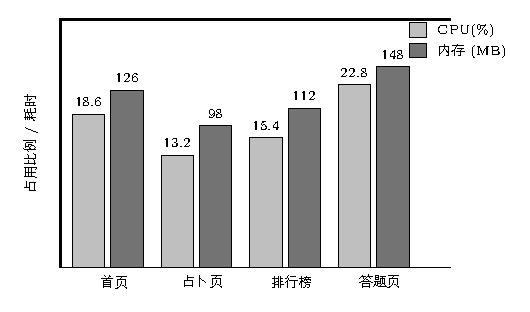
\includegraphics[width=0.86\textwidth]{figures/fig-perf.pdf}
  \caption{各页面性能测试图}
  \label{fig:perf}
\end{figure}

由测试结果可以看出，四个主要页面的 CPU 占用率均低于 25\%，内存占用均低于 150\,MB，页面平均加载时间在 1\,s 以内，各项性能指标均满足轻应用类小程序的上线要求。
